\section{THE PANOPTES ARCHITECTURE}
\label{sec:panoptes-architecture}

The proposed reference architecture, PANOPTES, was implemented integrating the ``Three Pillars'' of observability into a cohesive stack. Unlike proprietary solutions that rely on black-box agents, PANOPTES is built entirely on CNCF open-source projects.

\begin{figure}[htbp]
  \centering
  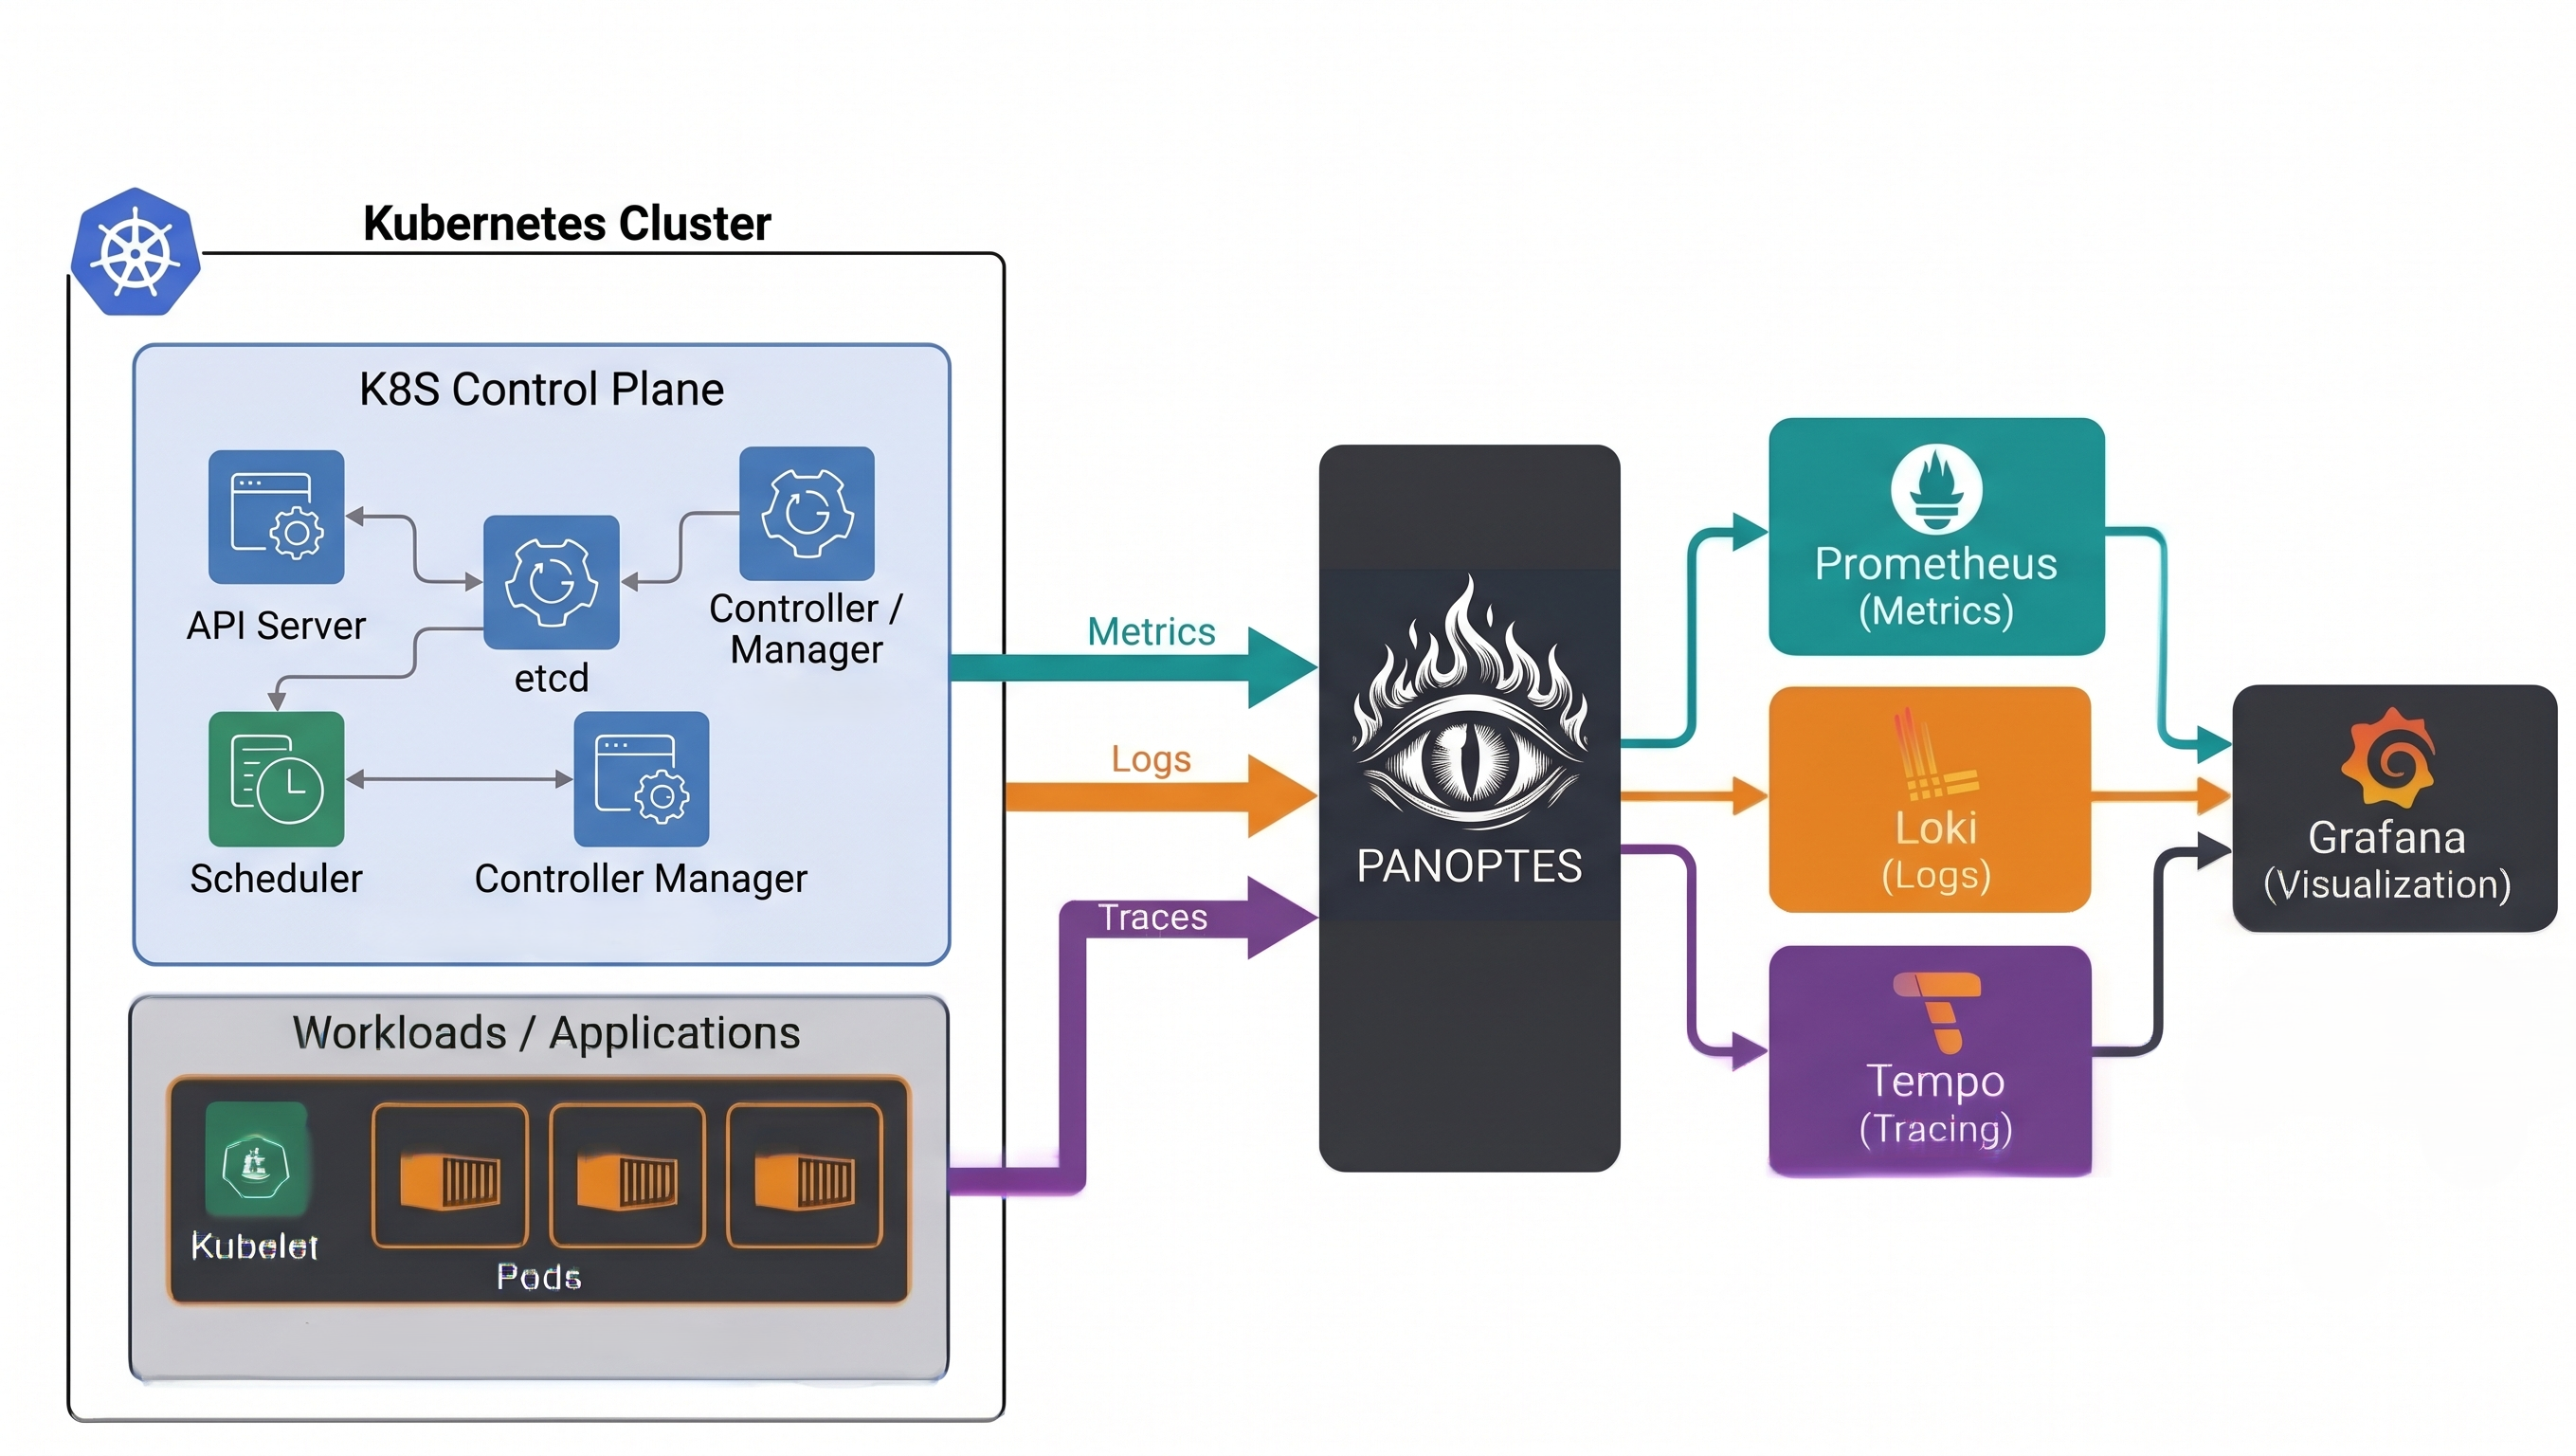
\includegraphics[width=1.0\textwidth]{images/experiment/panoptes_architecture.png}
  \caption{The PANOPTES Reference Architecture for Kubernetes Observability.}
  \label{fig:panoptes_arch}
\end{figure}

As illustrated in Figure \ref{fig:panoptes_arch}, the architecture is systematically divided into three main layers: Signal Generation (OTel), Storage Backends, and the Visualization Layer.